\documentclass[10pt]{article}
% \usepackage[pdftex]{graphicx, color}
\usepackage{listings}
\usepackage{mathtools} 
\usepackage{tikz}
\usepackage{hyperref}
\usepackage{ctex}
\usepackage{color}



\usetikzlibrary{automata,positioning}

\headheight 8pt \headsep 20pt \footskip 30pt
\textheight 9in \textwidth 6.5in
\oddsidemargin 0in \evensidemargin 0in
\topmargin -.35in

\newcommand {\pts}[1]{({\bf #1 pts})}
\lstset{basicstyle=\small\ttfamily,breaklines=true}

\begin{document}

\begin{center}
    \Large CS131 Compilers: Writing Assignment 1\\Due March 13, 2022
\end{center}

\begin{center}
    %% Change this:
    \LARGE 田皓原 - 2020533013
\end{center}


This assignment asks you to prepare written answers to questions on
regular languages, finite automata, and lexical analysis.  Each of the
questions has a short answer.  You may discuss this assignment with
other students and work on the problems together.  However, your
write-up should be your own individual work and you should indicate in your submission who you worked
with, if applicable.  Written assignments are submitted on \textbf{Gradescope}.
You should use the Latex template provided at the course web site to write your solution and use the \emph{tikz} package to draw
automata, and \textbf{all the submission that use other method to draw the graph will be deducted all the scores of the question}.

\begin{center}
    %% Change this:
    I worked with: nobody
\end{center}


\begin{enumerate}
    \item \pts{$1\times3 = 3$} For each of the follow prompts, write any non-empty sentence:
          \begin{enumerate}
              \item[\textbf{a}.] Name one reason why you would like to learn in this class.
              \item[\textbf{b}.] Write a question you would like the professor to answer 1 on any topic, from personal opinions to the class material and the teaching assistant to answer 1 in the discussion part.
              \item[\textbf{c}.] What do you expect from this class.
          \end{enumerate}
          \textcolor{blue}{
              \textbf{Answer}
              \begin{enumerate}
                  \item When talking about duplicate checking of code, TA of cs100 said that you would never simiply change the names of variables and regard it as totally different from the other code, when you actually have learnt Compilers. (now i know they are all 'identifier's after lexical analysis.) I found it interesting in learning the underlying, deepening my understanding.
                  \item I don't have rudimentary knowledge base yet in computer underlying, what basic knowledge am I supposed to master, as a beginer, or is there some book or website recommended that I can learn some related simple basis by myself. Thanks!
                  \item Just learn more about compilers, how it works, how to implement, how to optimize.
              \end{enumerate}
          }


    \item \pts{$1\times 3=3$} Regular expression.
          \begin{enumerate}
              \item[\textbf{a}.] Strings over the alphabet $\Sigma$ = \{$a$, $b$\} that contains at most two a’s, and at least three b’s.
              \item[\textbf{b}.] Strings over the alphabet $\Sigma$ = \{$a$, $b$\} that do not end in a double letter(e.g. $aa$ or $bb$).
              \item[\textbf{c}.] Strings over the alphabet $\Sigma$ = \{$a$, $b$, $c$\} that $a$ will not appear adjacent.
          \end{enumerate}
          \textcolor{blue}{
              \textbf{Answer}
              \begin{enumerate}
                  %   \item $((\epsilon|a)((ab|ba)b|bba)b | (\epsilon|a)bbbb^*(\epsilon|a) |(ab|ba)^2|aabb|bbaa)b^*$
                  \item $(bbb|abbb|babb|bbab|bbbb^*a|aabbb|ababb|abbab|abbbb^*a|baabb|babab|babbb^*a|bbaab|bbabb^*a|bbbb^*ab^*a)b^*$
                  \item $(a|b)^*(ab|ba)|a|b|\epsilon$
                  \item $(b|c)^*(a(b|c)^+)^*a?(b|c)^*$
              \end{enumerate}
          }
    \item \pts{$2\times 3=6$} Describe the strings which the following automata accept.
          \begin{enumerate}
              \item[] \textbf{a}.
                  \\
                  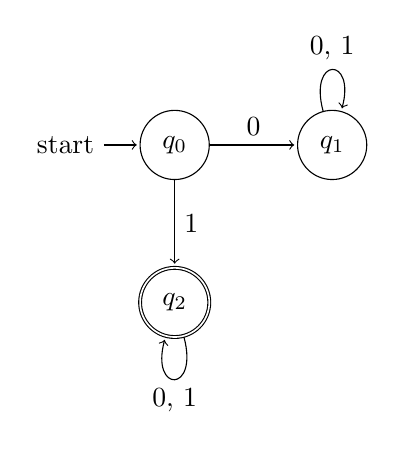
\begin{tikzpicture}[shorten >=1pt,node distance=2cm,on grid,auto]
                      \node[state, initial] (q_0) {$q_0$};
                      \node[state] (q_1) [right=of q_0] {$q_1$};
                      \node[state, accepting] (q_2) [below=of q_0] {$q_2$};
                      \path[->]
                      (q_0) edge node {0} (q_1)
                      edge node {1} (q_2)
                      (q_1) edge [loop above] node {0, 1} (q_1)
                      (q_2) edge [loop below] node {0, 1} (q_2);
                  \end{tikzpicture}

              \item[] \textbf{b}.
                  \\
                  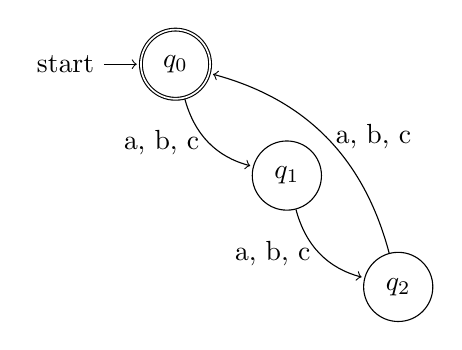
\begin{tikzpicture}[shorten >=1pt,node distance=2cm,on grid,auto]
                      \node[state, initial, accepting] (q_0) {$q_0$};
                      \node[state] (q_1) [below right=of q_0] {$q_1$};
                      \node[state] (q_2) [below right=of q_1] {$q_2$};
                      \path[->]
                      (q_0) edge [bend right] node [left]{a, b, c} (q_1)
                      (q_1) edge [bend right] node [left]{a, b, c} (q_2)
                      (q_2) edge [bend right] node [right]{a, b, c} (q_0);
                  \end{tikzpicture}
              \item[] \textbf{c}.
                  \\
                  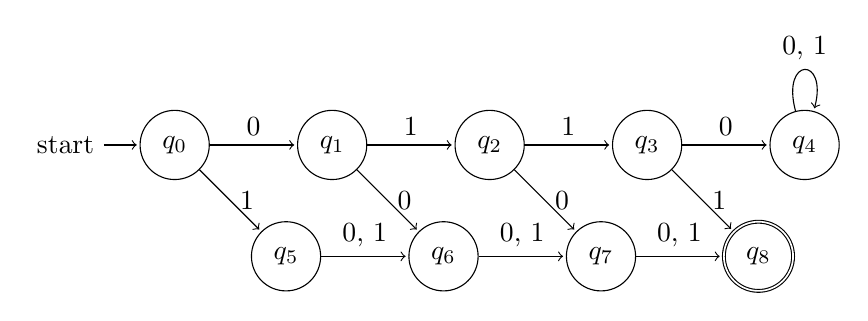
\begin{tikzpicture}[shorten >=1pt,node distance=2cm,on grid,auto]
                      \node[state, initial] (q_0) {$q_0$};
                      \node[state] (q_1) [right=of q_0] {$q_1$};
                      \node[state] (q_2) [right=of q_1] {$q_2$};
                      \node[state] (q_3) [right=of q_2] {$q_3$};
                      \node[state] (q_4) [right=of q_3] {$q_4$};
                      \node[state] (q_5) [below right=of q_0] {$q_5$};
                      \node[state] (q_6) [below right=of q_1] {$q_6$};
                      \node[state] (q_7) [below right=of q_2] {$q_7$};
                      \node[state, accepting] (q_8) [below right=of q_3] {$q_8$};
                      \path[->]
                      (q_0) edge node [above]{0} (q_1)
                      edge node [right]{1} (q_5)
                      (q_1) edge node [above]{1} (q_2)
                      edge node [right]{0} (q_6)
                      (q_2) edge node [above]{1} (q_3)
                      edge node [right]{0} (q_7)
                      (q_3) edge node [above]{0} (q_4)
                      edge node [right]{1} (q_8)
                      (q_4) edge [loop above] node {0, 1} (q_4)
                      (q_5) edge node [above]{0, 1} (q_6)
                      (q_6) edge node [above]{0, 1} (q_7)
                      (q_7) edge node [above]{0, 1} (q_8);
                  \end{tikzpicture}
          \end{enumerate}
          \textcolor{blue}{
              \textbf{Answer}
              \begin{enumerate}
                  \item Strings over the alphabet $\Sigma$ = \{$0$, $1$\} that start with 1.
                  \item Strings over the alphabet $\Sigma$ = \{$a$, $b$, $c$\} whose length is a multiple of three.
                  \item Strings over the alphabet $\Sigma$ = \{$0$, $1$\} whose length is four except $0110$.
              \end{enumerate}
          }
    \item \pts{$2\times 3=6$} Convert the following regular expression to minimized DFA, the process is required.
          \begin{enumerate}
              \item[\textbf{a}.] $a(b|c)^{*}$
              \item[\textbf{b}.] $((\epsilon|a)|b^{*})^{*}$
              \item[\textbf{c}.] $(a|b)^{*}abb(a|b)^{*}$
          \end{enumerate}
          \textcolor{blue}{
              \textbf{Answer}
              \begin{enumerate}
                  \item $a(b|c)^*\#$\\
                        $1~2~3~~~4$\\
                        $followpos(1)=\{2,3,4\}\\
                            followpos(2)=\{2,3,4\}\\
                            followpos(3)=\{2,3,4\}\\
                            followpos(4)=\{\}$\\
                        $S_0=firstpos(root)=\{1\}$\\
                        mark $S_0$\\
                        $a:followpos(1)=\{2,3,4\}=S_1,~move(S_0,a)=S_1$\\
                        mark $S_1$\\
                        $b:followpos(2)=\{2,3,4\}=S_1,~move(S_1,b)=S_1\\
                            c:followpos(3)=\{2,3,4\}=S_1,~move(S_1,c)=S_1$\\
                        initial state: $S_0$\\
                        accepting state; $S_1$\\
                        \begin{tikzpicture}[shorten >=1pt,node distance=2cm,on grid,auto]
                            \node[state, initial] (S_0) {$S_0$};
                            \node[state, accepting] (S_1) [right=of q_0] {$S_1$};
                            \path[->]
                            (S_0) edge node {a} (S_1)
                            (S_1) edge [loop above] node {b, c} (S_1);
                        \end{tikzpicture}
                  \item $((\epsilon|a)b^*)^*\#$\\
                        $~~~~~~1~2~~~~3$\\
                        $followpos(1)=\{1,2,3\}\\
                            followpos(2)=\{1,2,3\}\\
                            followpos(3)=\{\}$\\
                        $S_0=firstpos(root)=\{1,2,3\}$\\
                        mark $S_0$\\
                        $a:followpos(1)=\{1,2,3\}=S_0,~move(S_0,a)=S_0\\
                            b:followpos(2)=\{1,2,3\}=S_0,~move(S_0,b)=S_0$\\
                        initial state:$S_0$\\
                        accepting state:$S_0$\\
                        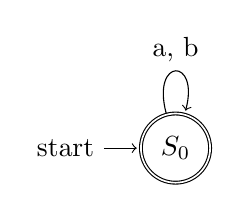
\begin{tikzpicture}[shorten >=1pt,node distance=2cm,on grid,auto]
                            \node[state, initial, accepting] (S_0) {$S_0$};
                            \path[->]
                            (S_0) edge [loop above] node {a, b} (S_0);
                        \end{tikzpicture}
                  \item $(a|b)^{*}abb(a|b)^{*}\#$\\
                        $~~1~2~~345~6~7~~~8$\\
                        $followpos(1)=\{1,2,3\}\\
                            followpos(2)=\{1,2,3\}\\
                            followpos(3)=\{4\}\\
                            followpos(4)=\{5\}\\
                            followpos(5)=\{6,7,8\}\\
                            followpos(6)=\{6,7,8\}\\
                            followpos(7)=\{6,7,8\}\\
                            followpos(8)=\{\}\\$
                        $S_0=firstpos(root)=\{1,2,3\}$\\
                            mark $S_0$\\
                        $a:followpos(1)\cup followpos(3)=\{1,2,3,4\}=S_1,~move(S_0,a)=S_1$\\
                        $b:followpos(2)=\{1,2,3\}=S_0,~move(S_0,b)=S_0$\\
                            mark $S_1$\\
                        $a:followpos(1)\cup followpos(3)=\{1,2,3,4\}=S_1,~move(S_1,a)=S_1\\
                        b:followpos(2)\cup followpos(4)=\{1,2,3,5\}=S_2,~move(S_1,b)=S_2$\\
                            mark $S_2$\\
                        $a:followpos(1)\cup followpos(3)=\{1,2,3,4\}=S_1,~move(S_2,a)=S_1\\
                        b:followpos(2)\cup followpos(5)=\{1,2,3,6,7,8\}=S_3,~move(S_2,b)=S_3$\\
                            mark $S_3$\\
                        $a:followpos(1)\cup followpos(3)\cup followpos(6)=\{1,2,3,4,6,7,8\}=S_4,~move(S_3,a)=S_4\\
                        b:followpos(2)\cup followpos(7)=\{1,2,3,6,7,8\}=S_3,~move(S_3,b)=S_3$\\
                            mark $S_4$\\
                        $a:followpos(1)\cup followpos(3)\cup followpos(6)=\{1,2,3,4,6,7,8\}=S_4,~move(S_4,a)=S_4\\
                        b:followpos(2)\cup followpos(4)\cup followpos(7)=\{1,2,3,5,6,7,8\}=S_5,~move(S_4,b)=S_5$\\
                            mark $S_5$\\
                        $a:followpos(1)\cup followpos(3)\cup followpos(6)=\{1,2,3,4,6,7,8\}=S_4,~move(S_5,a)=S_4\\
                        b:followpos(2)\cup followpos(5)\cup followpos(7)=\{1,2,3,6,7,8\}=S_3,~move(S_5,b)=S_3$\\
                            initial state:$S_0$\\
                            accepting state:$S_3,S_4,S_5$\\
                            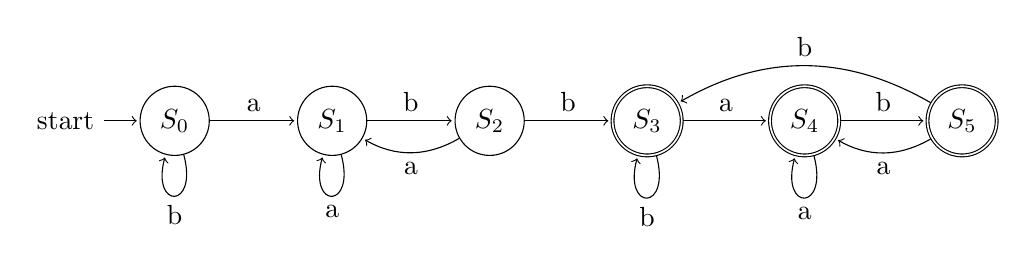
\begin{tikzpicture}[shorten >=1pt,node distance=2cm,on grid,auto]
                                \node[state, initial] (S_0) {$S_0$};
                                \node[state] (S_1) [right=of S_0] {$S_1$};
                                \node[state] (S_2) [right=of S_1] {$S_2$};
                                \node[state, accepting] (S_3) [right=of S_2] {$S_3$};
                                \node[state, accepting] (S_4) [right=of S_3] {$S_4$};
                                \node[state, accepting] (S_5) [right=of S_4] {$S_5$};
                                \path[->]
                                (S_0) edge [loop below] node {b} (S_0)
                                edge node {a} (S_1)
                                (S_1) edge [loop below] node {a} (S_1)
                                edge node {b} (S_2)
                                (S_2) edge node {b} (S_3)
                                edge [bend left] node {a} (S_1)
                                (S_3) edge node {a} (S_4)
                                edge [loop below] node {b} (S_3)
                                (S_4) edge node {b} (S_5)
                                edge [loop below] node {a} (S_4)
                                (S_5) [bend right] edge node [above] {b} (S_3)
                                edge [bend left] node {a} (S_4);
                            \end{tikzpicture}\\
                            Affere minimizing,\\
                            initial state:$S_0$\\
                            accepting state:$S_3$\\
                        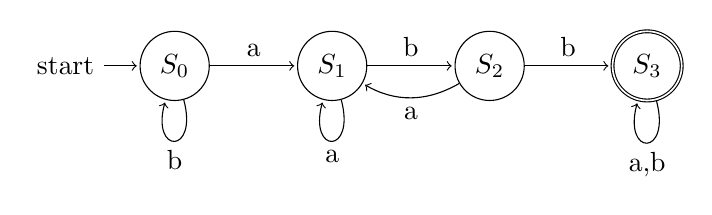
\begin{tikzpicture}[shorten >=1pt,node distance=2cm,on grid,auto]
                            \node[state, initial] (S_0) {$S_0$};
                            \node[state] (S_1) [right=of S_0] {$S_1$};
                            \node[state] (S_2) [right=of S_1] {$S_2$};
                            \node[state, accepting] (S_3) [right=of S_2] {$S_3$};
                            \path[->]
                            (S_0) edge [loop below] node {b} (S_0)
                            edge node {a} (S_1)
                            (S_1) edge [loop below] node {a} (S_1)
                            edge node {b} (S_2)
                            (S_2) edge node {b} (S_3)
                            edge [bend left] node {a} (S_1)
                            (S_3) edge [loop below] node {a,b} (S_3);
                        \end{tikzpicture}
              \end{enumerate}
          }
    \item \pts{$2\times 3=6$} Convert the following NFAs to minimized DFAs, the process is not required.
          \begin{enumerate}
              \item[] \textbf{a}
                  \\
                  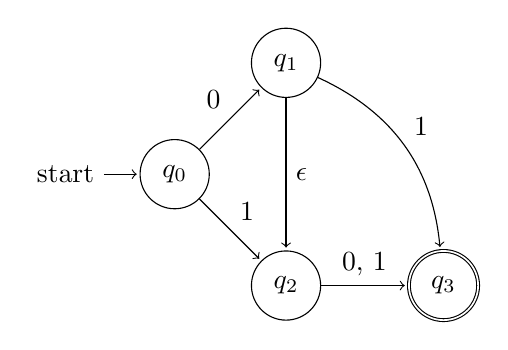
\begin{tikzpicture}[shorten >=1pt,node distance=2cm,on grid,auto]
                      \node[state, initial] (q_0) {$q_0$};
                      \node[state] (q_1) [above right=of q_0] {$q_1$};
                      \node[state] (q_2) [below right=of q_0] {$q_2$};
                      \node[state, accepting] (q_3) [right=of q_2] {$q_3$};
                      \path[->]
                      (q_0) edge node {0} (q_1)
                      edge node {1} (q_2)
                      (q_1) edge node {$\epsilon$} (q_2)
                      edge [bend left] node {1} (q_3)
                      (q_2) edge node {0, 1} (q_3);
                  \end{tikzpicture}
              \item[] \textbf{b}. Question 2.a.
              \item[] \textbf{c}. Question 2.c.
          \end{enumerate}
          \textcolor{blue}{
              \textbf{Answer}
              \begin{enumerate}
                  \item \tikzpicture[shorten >=1pt,node distance=2cm,on grid,auto]
                        \node[state, initial] (q_0) {$q_0$};
                        \node[state] (q_1) [right=of q_0] {$q_1$};
                        \node[state, accepting] (q_2) [right=of q_1] {$q_2$};
                        \path[->]
                        (q_0) edge node {0,1} (q_1)
                        (q_1) edge node {0,1} (q_2);
                        \endtikzpicture
                  \item
                        \tikzpicture[shorten >=1pt,node distance=2cm,on grid,auto]
                        \node[state, initial, accepting] (q_0) {$q_0$};
                        \node[state, accepting] (q_1) [above right=of q_0] {$q_1$};
                        \node[state, accepting] (q_2) [below right=of q_0] {$q_2$};
                        \node[state] (q_3) [above right=of q_1] {$q_3$};
                        \node[state] (q_4) [below right=of q_2] {$q_4$};
                        \path[->]
                        (q_0) edge node {a} (q_1)
                        edge node [below] {b} (q_2)
                        (q_1) edge node {a} (q_3)
                        edge node {b} (q_2)
                        (q_2) edge node {b} (q_4)
                        edge [bend left] node {a} (q_1)
                        (q_3) edge [loop above] node {a} (q_3)
                        edge [bend left] node [below] {b} (q_2)
                        (q_4) edge [loop below] node {b} (q_3=4)
                        edge [bend right] node [above] {a} (q_1);
                        \endtikzpicture
                  \item \tikzpicture[shorten >=1pt,node distance=2cm,on grid,auto]
                        \node[state, initial, accepting] (q_0) {$q_0$};
                        \node[state, accepting] (q_1) [right=of q_0] {$q_1$};
                        \path[->]
                        (q_0) edge node {a} (q_1)
                        edge [loop above] node {b,c} (q_0)
                        (q_1) edge [bend left] node {b,c} (q_0);
                        \endtikzpicture
              \end{enumerate}
          }

    \item \pts{$10$} Let $L$ be a language over $\Sigma=\{a, b, c\}$.\\
          String $w$ is in $L$ if and only if $w$ is of the form $w$ = $x^{n}s$ where $x$ is $a$ or $b$ or $c$, $n$ $\ge$ 0, and $s$ is a string that does not contain $x$ as a substring.
          Here, $x^n$ denotes $x$ being repeated $n$ times. You can imagine $w$ as a string with a head consisting of a character repeated 0 or more times and said
          character does not appears in the tail of $w$. \\
          Examples of strings in $L$: $\underline{c}abab$, $\underline{bbb}$, $\underline{bb}$aaac. \\
          Examples of strings not in $L$: $\underline{b}$aaa$\underline{b}$c, $\underline{c}$ab$\underline{c}$ab. \\
          Draw an NFA for $L$. Your solution should not have more than \textbf{10} states.\\
          \textcolor{blue}{
              \textbf{Answer}\\
              \tikzpicture[shorten >=1pt,node distance=3cm,on grid,auto]
              \node[state, initial, accepting] (q_0) {$q_0$};
              \node[state, accepting] (q_1) [above right=of q_0] {$q_1$};
              \node[state, accepting] (q_2) [right=2.122cm of q_0] {$q_2$};
              \node[state, accepting] (q_3) [below right=of q_0] {$q_3$};
              \node[state, accepting] (q_4) [right=of q_1] {$q_4$};
              \node[state, accepting] (q_5) [right=of q_2] {$q_5$};
              \node[state, accepting] (q_6) [right=of q_3] {$q_6$};
              \node[state, accepting] (q_7) [right=of q_4] {$q_7$};
              \node[state, accepting] (q_8) [right=of q_5] {$q_8$};
              \node[state, accepting] (q_9) [right=of q_6] {$q_9$};
              \path[->]
              (q_0) edge node {a} (q_1)
              edge node {b} (q_2)
              edge node {c} (q_3)
              (q_1) edge [loop above] node {a} (q_1)
              edge node {b} (q_5)
              edge node {c} (q_6)
              (q_2) edge [loop above] node {b} (q_2)
              edge node {a} (q_4)
              edge node {c} (q_6)
              (q_3) edge [loop above] node {a} (q_3)
              edge node {b} (q_5)
              edge node {a} (q_4)
              (q_4) edge [loop above] node {a} (q_4)
              edge node {b} (q_9)
              edge node {a} (q_8)
              (q_5) edge [loop above] node {b} (q_5)
              edge node {c} (q_7)
              edge node {a} (q_9)
              (q_6) edge [loop above] node {c} (q_6)
              edge node {b} (q_7)
              edge node {a} (q_8)
              (q_7) edge [loop above] node {b,c} (q_7)
              (q_8) edge [loop above] node {a,c} (q_8)
              (q_9) edge [loop above] node {a,b} (q_9);
              \endtikzpicture
          }

    \item \pts{$10$} Draw the NFA for the set of all strings over the alphabet $\Sigma = \{a,b\}$, where both $a$ and $b$ occur even times.

          Examples of strings that should be accepted by this NFA: abbabbbbaa, baabaaabaaaaab.

          Examples of strings that should \textbf{not} be accepted: ababb, abbbabba.

          \textcolor{blue}{
              \textbf{Answer}\\
              The regular expression should be $(aa|bb)^*((ab|ba)(aa|bb)^*(ab|ba)(aa|bb)^*)^*$\\
              Since the NFA can be so big, I would like to show it with some equivalent symbols.\\
              Mark $A$ equivalent to the following NFA (corresponding to regular expression $(aa|bb)^*$):\\
              \tikzpicture[shorten >=1pt,node distance=2cm,on grid,auto]
              \node[state, initial] (q_0) {$q_0$};
              \node[state] (q_1) [right=of q_0] {$q_1$};
              \node[state] (q_2) [above right=of q_1] {$q_2$};
              \node[state] (q_3) [below right=of q_1] {$q_3$};
              \node[state] (q_4) [right=of q_2] {$q_4$};
              \node[state] (q_5) [right=of q_3] {$q_5$};
              \node[state] (q_6) [right=of q_4] {$q_6$};
              \node[state] (q_7) [right=of q_5] {$q_7$};
              \node[state] (q_8) [below right=of q_6] {$q_8$};
              \node[state, accepting] (q_9) [right=of q_8] {$q_9$};
              \path[->]
              (q_0) edge node {$\epsilon$} (q_1)
              edge [bend left=50] node {$\epsilon$} (q_9)
              (q_1) edge node {$\epsilon$} (q_2)
              edge node {$\epsilon$} (q_3)
              (q_2) edge node {a} (q_4)
              (q_3) edge node {b} (q_5)
              (q_4) edge node {a} (q_6)
              (q_5) edge node {b} (q_7)
              (q_6) edge node {$\epsilon$} (q_8)
              (q_7) edge node {$\epsilon$} (q_8)
              (q_8) edge node {$\epsilon$} (q_9)
              edge [bend left=100] node {$\epsilon$} (q_1);
              \endtikzpicture\\
              Mark $B$ equivalent to the following NFA (corresponding to regular expression $(ab|ba)$):\\
              \tikzpicture[shorten >=1pt,node distance=2cm,on grid,auto]
              \node[state, initial] (q_1) {$q_0$};
              \node[state] (q_2) [above right=of q_1] {$q_1$};
              \node[state] (q_3) [below right=of q_1] {$q_2$};
              \node[state] (q_4) [right=of q_2] {$q_3$};
              \node[state] (q_5) [right=of q_3] {$q_4$};
              \node[state] (q_6) [right=of q_4] {$q_5$};
              \node[state] (q_7) [right=of q_5] {$q_6$};
              \node[state, accepting] (q_8) [below right=of q_6] {$q_7$};
              \path[->]
              (q_1) edge node {$\epsilon$} (q_2)
              edge node {$\epsilon$} (q_3)
              (q_2) edge node {a} (q_4)
              (q_3) edge node {b} (q_5)
              (q_4) edge node {b} (q_6)
              (q_5) edge node {a} (q_7)
              (q_6) edge node {$\epsilon$} (q_8)
              (q_7) edge node {$\epsilon$} (q_8);
              \endtikzpicture\\
              So we can get the NFA for $(aa|bb)^*((ab|ba)(aa|bb)^*(ab|ba)(aa|bb)^*)^*$ in terms of A and B:\\
              \tikzpicture[shorten >=1pt,node distance=1.5cm,on grid,auto]
              \node[state, initial] (q_0) {$q_0$};
              \node[state] (q_1) [right=of q_0] {$A$};
              \node[state] (q_2) [right=of q_1] {$q_2$};
              \node[state] (q_3) [right=of q_2] {$q_3$};
              \node[state] (q_4) [right=of q_3] {$B$};
              \node[state] (q_5) [right=of q_4] {$A$};
              \node[state] (q_6) [right=of q_5] {$B$};
              \node[state] (q_7) [right=of q_6] {$A$};
              \node[state] (q_8) [right=of q_7] {$q_8$};
              \node[state, accepting] (q_9) [right=of q_8] {$q_9$};
              \path[->]
              (q_0) edge node {$\epsilon$} (q_1)
              (q_1) edge node {$\epsilon$} (q_2)
              (q_2) edge node {$\epsilon$} (q_3)
              edge [bend left] node {$\epsilon$} (q_9)
              (q_3) edge node {$\epsilon$} (q_4)
              (q_4) edge node {$\epsilon$} (q_5)
              (q_5) edge node {$\epsilon$} (q_6)
              (q_6) edge node {$\epsilon$} (q_7)
              (q_7) edge node {$\epsilon$} (q_8)
              (q_8) edge node {$\epsilon$} (q_9)
              edge [bend left] node {$\epsilon$} (q_3);
              \endtikzpicture\\
          }
    \item \pts{$10$} Give the simplest description you can of the language described by the DFA below:
          \\
          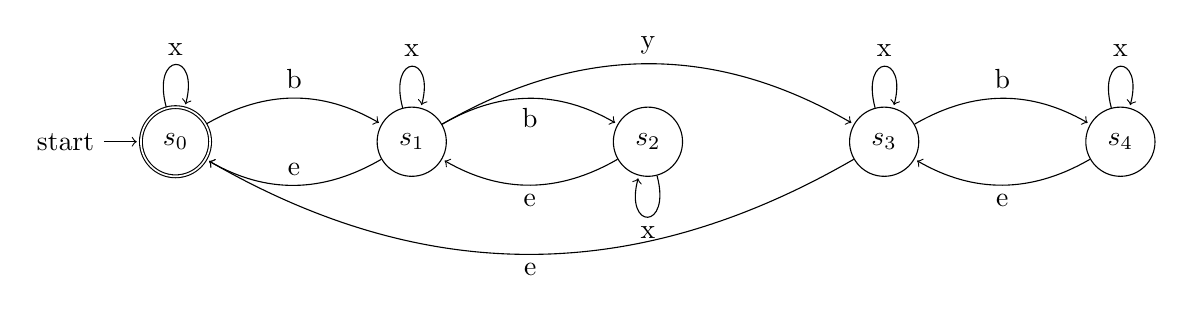
\begin{tikzpicture}[shorten >=1pt,node distance=3cm,on grid,auto]
              \node[state,initial,accepting](s_0){$s_0$};
              \node[state](s_1)[right of= s_0]{$s_1$};
              \node[state](s_2)[right of= s_1]{$s_2$};
              \node[state](s_3)[right of=s_2]{$s_3$};
              \node[state](s_4)[right of=s_3]{$s_4$};
              \path[->]
              (s_0)[loop above]edge node{x}(s_0)
              edge[bend left] node{b}(s_1)
              (s_1)[loop above]edge node{x}(s_1)
              edge[bend left] node[below]{b}(s_2)
              edge[bend left] node[above]{e}(s_0)
              edge[bend left] node[above]{y}(s_3)
              (s_2)[loop below]edge node{x}(s_2)
              edge[bend left] node[below]{e}(s_1)
              (s_3)[loop above]edge node{x}(s_3)
              edge[bend left] node{b}(s_4)
              edge[bend left] node[below]{e}(s_0)
              (s_4)[loop above]edge node{x}(s_4)
              edge[bend left] node[below]{e}(s_3);
          \end{tikzpicture}

          \textcolor{blue}{
              \textbf{Answer}\\
              My idea:\\
              I found that every state has a self loop with x, and all edge b go right, all edge e go left.
              Here I would like to declare a system that, each state has a state number, each edge b indicates $+1$ on the state numbers from one state to another, and edge e $-1$, edge x $+0$.
              By calculation, I found that this system is consistent with the rule. The state number from $s_0$ to $s_4$ are respectively $0,1,2,1,2$. y acts as a spliter of the string, and is defined as $+0$ in this system.\\
              Then let's extract some features in this system:
              \begin{enumerate}
                  \item Since there is only one accepting state $s_0$ whose state number is 0, there must be equal number of edge b and e in the string.
                  \item Since egde y is from $s_1$ to $s_3$, both have state number $1$. So if we split the string into pieces with y, the number of b must be the number of e plus one before each y, and the number of e must be the number of b plus one after each y. Concluding that, the number of b equals 1 + the number of e before the first y, the number of e equals 1 + the number of b after the last y, and between two y's, the number of e and b are equal.
                  \item Since the state number can be only $0,1,2$, so the number of b (denotes $|b|$) and the number of e (denotes $|e|$) in every substring from the begining should follow: $|e|\leq |b|\leq |e|+2$.
                  \item x can be anywhere in the string.
              \end{enumerate}
              So, my final answer is:\\
              Strings over the alphabet $\Sigma$ = \{$x$, $y$,$b$,$e$\} that,\\
              from the begining till every character in the string, the number of $b$ (denotes $|b|$) and the number of $e$ (denotes $|e|$) should keep: $|e|\leq |b|\leq |e|+2$;\\
              $|b|=|e|+1$ before the first $y$, $|e|=|b|+1$ after the last $y$, $|e|=|b|$ between all $y$'s; specially $|e|=|b|$ if there is no $y$;\\
              $x$ can be anywhere in the string.
          }

\end{enumerate}


\end{document}


